\documentclass[12pt]{article}
\usepackage{amsfonts,amssymb,float,amsmath}
\usepackage{algorithmic}
\usepackage{graphicx, siunintx}
\usepackage{textcomp}
\usepackage{xcolor}
\usepackage{txfonts}
\usepackage{multicol}
\usepackage{listings}
\usepackage{enumitem}
\usepackage{mathtools}
\usepackage{gensymb}
\usepackage{comment}
\usepackage[breaklinks=true]{hyperref}
\usepackage{tkz-euclide} 
\usepackage{listings}
\usepackage{gvv}                       
\usepackage{gvv-book}
%\def\inputGnumericTable{}                             
\usepackage{color}                                            
\usepackage{array}                                            
\usepackage{longtable}                                       
\usepackage{calc}                                             
\usepackage{multirow}                                         
\usepackage{hhline}                                           
\usepackage{ifthen}                                           
\usepackage{lscape}
\newcommand{\BEQA}{\begin{eqnarray}}
\newcommand{\EEQA}{\end{eqnarray}}
%\newcommand{\define}{\stackrel{\triangle}{=}}
\theoremstyle{remark}
\newtheorem{rem}{Remark}
\parindent 0px
\pagenumbering{gobble}
\begin{document}
\title{\vspace{-5cm}Gate paper 2023-XH}
\author{Ayush Sunil Labhade}
\date{AI25Btech11002}
\maketitle

\begin{flushright}Humanities and Social Sciences-Linguistics (XH-C3)\end{flushright}
\begin{flushleft}General Aptitude \textbf{\brak{GA}} \\[5pt]
\textbf{\item Q.1 - Q.5 Carry ONE mark each}\end{flushleft}
\begin{enumerate}
%Q.1
\item Rafi told Mary, “I am thinking of watching a film this weekend.”
The following reports the above statement in indirect speech:
Rafi told Mary that he \_\_\_\_\_\_\_ of watching a film that weekend.
\begin{enumerate} \begin{multicols}{2}
\item thought
\item is thinking
\item am thinking
\item was thinking
\end{multicols} \end{enumerate}
\hfill\brak{GATE \ XH \ 2023}
%Q.2
\item Permit : \_\_\_\_\_\_\_ :: Enforce : Relax
\brak{By word meaning}\newline
\begin{enumerate} \begin{multicols}{4} 
\item Allow
\item Forbid
\item License
\item Reinforce
\end{multicols} \end{enumerate}
\hfill\brak{GATE \ XH \ 2023}
%Q.3
\item Given a fair six-faced dice where the faces are labelled ‘1’, ‘2’, ‘3’, ‘4’, ‘5’, and ‘6’, what is the probability of getting a ‘1’ on the first roll of the dice and a ‘4’ on the second roll?
\begin{enumerate} \begin{multicols}{4}
\item $\frac{1}{36}$
\item $\frac{1}{6}$
\item $\frac{5}{6}$
\item $\frac{1}{3}$
\end{multicols} \end{enumerate}
\hfill\brak{GATE \ XH \ 2023}
%Q.4
\item A recent survey shows that 65% of tobacco users were advised to stop consuming tobacco. The survey also shows that 3 out of 10 tobacco users attempted to stop using tobacco.
Based only on the information in the above passage, which one of the following options can be logically inferred with certainty?
\begin{enumerate}
\item A majority of tobacco users who were advised to stop consuming tobacco made an attempt to do so.
\item A majority of tobacco users who were advised to stop consuming tobacco did not attempt to do so.
\item Approximately 30% of tobacco users successfully stopped consuming tobacco.
\item Approximately 65% of tobacco users successfully stopped consuming tobacco.
\end{enumerate}
\hfill\brak{GATE \ XH \ 2023}
%Q.5
\item How many triangles are present in the given figure?
\begin{figure}[H]
\centering
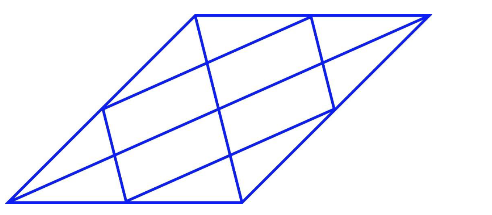
\includegraphics[width=0.4\textwidth]{Figs/Q5.png}
\caption{}
\label{fig:3.1}
\end{figure}
\begin{enumerate} \begin{multicols}{4}
\item 12
\item 16
\item 20
\item 24
\end{multicols} \end{enumerate}
\hfill\brak{GATE \ XH \ 2023}
\newpage
\textbf{Q.6- Q.10 Carry TWO marks Each}
%Q.6
\item Students of all the departments of a college who have successfully completed the registration process are eligible to vote in the upcoming college elections. However, by the time the due date for registration was over, it was found that surprisingly none of the students from the Department of Human Sciences had completed the registration process. Based only on the information provided above, which one of the following sets of statement(s) can be logically inferred with certainty?
\begin{enumerate}
\item [(i)] All those students who would not be eligible to vote in the college elections would certainly belong to the Department of Human Sciences.
\item [(ii)] None of the students from departments other than Human Sciences failed to complete the registration process within the due time.
\item [(iii)] All the eligible voters would certainly be students who are not from the Department of Human Sciences.
\end{enumerate} 
\begin{enumerate} \begin{multicols}{4}
\item (i) and (ii) 
\item (i) and (iii) 
\item only (i)
\item only (iii) 
\end{multicols} \end{enumerate}
\hfill\brak{GATE \ XH \ 2023}
%Q.7
\item Which one of the following options represents the given graph?
\begin{figure}[H]
\centering
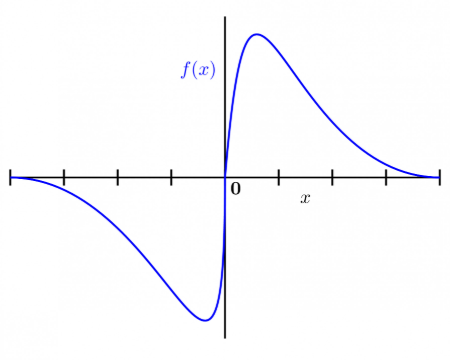
\includegraphics[width=0.5\textwidth]{Figs/Q7.png}
\caption{}
\label{fig:3.2}
\end{figure}
\begin{enumerate} \begin{multicols}{4}
\item $f(x)=x^22^{-|x|}$ 
\item $f(x)=x2^{-|x|}$
\item $f(x)=|x|2^{-x}$ 
\item $f(x)=x2^{-x}$
\end{multicols} \end{enumerate}
\hfill\brak{GATE \ XH \ 2023}
%Q.8
\item Which one of the options does NOT describe the passage below or follow from it?
We tend to think of cancer as a ‘modern’ illness because its metaphors are so modern. It is a disease of overproduction, of sudden growth, a growth that is unstoppable, tipped into the abyss of no control. Modern cell biology encourages us to imagine the cell as a molecular machine. Cancer is that machine unable to quench its initial command (to grow) and thus transform into an indestructible, self-propelled automaton.\\
\sbrak{Adapted from \textit{The Emperor of All Maladies} by Siddhartha Mukherjee}
\begin{enumerate}
\item It is a reflection of why cancer seems so modern to most of us.
\item It tells us that modern cell biology uses and promotes metaphors of machinery.
\item Modern cell biology encourages metaphors of machinery, and cancer is often imagined as a machine.
\item Modern cell biology never uses figurative language, such as metaphors, to describe or explain anything.
\end{enumerate}
\hfill\brak{GATE \ XH \ 2023}
%Q.9
\item The digit in the unit’s place of the product $3^{999} \times 7^{1000}$ is
\begin{enumerate} \begin{multicols}{4}
\item 7
\item 1
\item 3
\item 9
\end{multicols} \end{enumerate}
\hfill\brak{GATE \ XH \ 2023}
%Q.10
\item A square with sides of length 6 cm is given. The boundary of the shaded region is defined by two semi-circles whose diameters are the sides of the square, as shown. The area of the shaded region is \_\_\_\_ cm$^2$.
\begin{figure}[H]
\centering
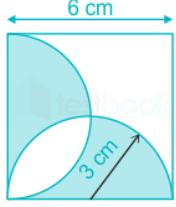
\includegraphics[width=0.3\textwidth]{Figs/Q10.png}
\caption{}
\label{fig:3.3}
\end{figure}
\begin{enumerate} \begin{multicols}{4} 
\item $6\pi$
\item 18 
\item 20 
\item $9\pi$ 
\end{multicols} \end{enumerate}
\hfill\brak{GATE \ XH \ 2023}
\newpage
\textbf{Reasoning and Comprehension(XH-B1)\newline 
XH-B1:Q11-Q17 Carry ONE mark Each}
%Q.11
\item Which word below best describes the idea of being both \textit{Spineless} and \textit{Cowardly}?
\begin{enumerate} \begin{multicols}{2}
\item Pusillanimous
\item Unctuous
\item Obsequious
\item Reticent
\end{multicols} \end{enumerate}
\hfill\brak{GATE \ XH \ 2023}
%Q.12
\item Choose the right preposition to fill up the blank:
The whole family got together \_\_\_\_\_\_\_ Diwali
\begin{enumerate} \begin{multicols}{4}
\item of
\item at
\item in
\item till
\end{multicols} \end{enumerate}
\hfill\brak{GATE \ XH \ 2023}
%Q.13
\item Select the correct option to fill in all the blanks to complete the passage:
The (i) \_\_\_\_\_\_\_\_\_ factor amid this turbulence has been the (ii) \_\_\_\_\_\_\_\_\_ of high-octane, action-oriented films such as RRR, K.G.F: Chapter 2 and Pushpa from film industries in the south of the country. Traditionally, films made in the south have done well in their own (iii) \_\_\_\_\_\_\_\_\_. But increasingly, their dubbed versions have performed well in the Hindi heartland, with collections (iv) \_\_\_\_\_\_\_\_\_ those of their Bollywood counterparts.
\begin{enumerate} 
\item (i) disheartening (ii) failure (iii) channels (iv) matching
\item (i) redeeming (ii) outperformance (iii) geographies (iv) eclipsing
\item (i) shocking (ii) underperformance (iii) cinemas (iv) below
\item (i) humbling (ii) bombing (iii) theatres (iv) falling behind
\end{enumerate}
\hfill\brak{GATE \ XH \ 2023}
%Q.14
\item The following passage consists of 6 sentences. The first and sixth sentences of the passage are at their correct positions, while the middle four sentences (represented by 2, 3, 4, and 5) are jumbled up. Choose the correct sequence of the sentences so that they form a coherent paragraph:
\begin{enumerate}
\item[1.] Most obviously, mobility is taken to be a geographical as well as a social phenomenon.
\item[2.] Much of the social mobility literature regarded society as a uniform surface and failed to register the geographical intersections of region, city and place, with the social categories of class, gender and ethnicity.
\item[3.] The existing sociology of migration is incidentally far too limited in its concerns to be very useful here.
\item[4.] Further, I am concerned with the flows of people within, but especially beyond, the territory of each society, and how these flows may relate to many different desires, for work, housing, leisure, religion, family relationships, criminal gain, asylum seeking and so on.
\item[5.] Moreover, not only people are mobile but so too are many ‘objects’.
\item[6.] I show that sociology’s recent development of a ‘sociology of objects’ needs to be taken further and that the diverse flows of objects across societal borders and their intersections with the multiple flows of people are hugely significant.
\end{enumerate}
\begin{enumerate} \begin{multicols}{4}
\item 3,2,5,4
\item 2,3,4,5
\item 5,4,3,2
\item 4,2,5,3
\end{multicols} \end{enumerate}
\hfill\brak{GATE \ XH \ 2023}
%Q.15
\item The population of a country increased by 5\% from 2020 to 2021. Then, the population decreased by 5\% from 2021 to 2022. By what percentage did the population change from 2020 to 2022?
\begin{enumerate} \begin{multicols}{4}
\item -0.25\%
\item 0\%
\item 2.5\%
\item 10.25\%
\end{multicols} \end{enumerate}
\hfill\brak{GATE \ XH \ 2023}
%Q.16
\item The words \textbf{Thin: Slim: Slender} are related in some way. Identify the correct option(s) that reflect(s) the same relationship: 
\begin{enumerate} \begin{multicols}{2}
\item Fat: Plump: Voluptuous
\item Short: Small: Petite
\item Tall: Taller: Tallest
\item Fair: Dark: Wheatish
\end{multicols} \end{enumerate}
\hfill\brak{GATE \ XH \ 2023}
%Q.17
\item A pandemic like situation hit the country last year, resulting in loss of human life and economic depression. To improve the condition of its citizens, the government made a series of emergency medical interventions and increased spending to revive the economy. In both these efforts, district administration authorities were actively involved. Which of the following action(s) are plausible?
\begin{enumerate}
\item In future, the government can make district administration authorities responsible for protecting health of citizens and reviving the economy.
\item The government may set up a task force to review the post pandemic situation and ascertain the effectiveness of the measures taken.
\item The government may set up a committee to formulate a pandemic management program to minimize losses to life and economy in future.
\item The government may take population control measures to minimize pandemic related losses in future.
\end{enumerate}
\hfill\brak{GATE \ XH \ 2023}
\newpage
\textbf{XH-B1:Q18-Q26 Carry TWO marks Each}
%Q.18
\item Six students, Arif, Balwinder, Chintu, David, Emon and Fulmoni appeared in the GATE-XH exam in 2022. Balwinder scores less than Chintu in XH-B1, but more than Arif in XH-C1. David scores more than Balwinder in XH-C1, and more than Chintu in XH-B1. Emon scores less than David, but more than Fulmoni in XH-B1. Fulmoni scores more than David in XH-C1. Arif scores less than Emon, but more than Fulmoni in XH-B1. Who scores highest in XH-B1?
\begin{enumerate} \begin{multicols}{4}
\item Fulmoni
\item Emon
\item David
\item Chintu
\end{multicols} \end{enumerate}
\hfill\brak{GATE \ XH \ 2023}
%Q.19
\item Select the correct relation between E and F.
$$ E = \frac{x}{1 + x} \quad \text{and} \quad F = \frac{-x}{1 - x} \quad x > 1 $$ 
\begin{enumerate} \begin{multicols}{4}
\item $E > F$ 
\item $E < F$ 
\item $E = F$ 
\item $E < -F$ 
\end{multicols} \end{enumerate}
\hfill\brak{GATE \ XH \ 2023}
%Q.20
\item A code language is formulated thus: Vowels in the original word are replaced by the next vowel from the list of vowels, A-E-I-O-U (For example, E is replaced by I and U is replaced by A). Consonants in the original word are replaced by previous consonant (For example, T is replaced by S and V is replaced by T). Then how does the word, GOODMORNING appear in the coded language?
\begin{enumerate} \begin{multicols}{2}
\item HUUFNUSPOPH
\item FIICLIQMEMF
\item FUUCLUQMOMF
\item HEEDATTACRH
\end{multicols} \end{enumerate}
\hfill\brak{GATE \ XH \ 2023}
%Q.21
\item The stranger is by nature no "owner of soil" -- soil not only in the physical, but also in the figurative sense of a life-substance, which is fixed, if not in a point in space, at least in an ideal point of the social environment. Although in more intimate relations, he may develop all kinds of charm and significance, as long as he is considered a stranger in the eyes of the other, he is not an "owner of soil." Restriction to intermediary trade, and often (as though sublimated from it) to pure finance, gives him the specific character of mobility. If mobility takes place within a closed group, it embodies that synthesis of nearness and distance which constitutes the formal position of the stranger. For, the fundamentally mobile person comes in contact, at one time or another, with every individual, but is not organically connected, through established ties of kinship, locality, and occupation, with any single one.
What assumptions can be made about the stranger from the passage above?
\begin{enumerate} 
\item The stranger can become an owner of soil through developing all kinds of charm in more intimate relations.
\item The stranger cannot become an owner of soil either in the physical or psychological sense.
\item The stranger can become an owner of soil through establishing ties of kinship and so on.
\item The stranger might become an owner of soil in the physical sense but not in the psychological.
\end{enumerate}
\hfill\brak{GATE \ XH \ 2023}
%Q.22
\item L is the only son of A and S. S has one sibling, B, who is married to L’s aunt, K. B is the only son of D. How are L and D related? Select the possible option(s):
\begin{enumerate} 
\item Grandchild and Paternal Grandfather
\item Grandchild and Maternal Grandfather
\item Grandchild and Paternal Grandmother
\item Grandchild and Maternal Grandmother
\end{enumerate}
\hfill\brak{GATE \ XH \ 2023}
%Q.23
\item Five segments of a sentence are given below. The first and fifth segments are at their correct positions, while the middle three segments (represented by 2, 3, and 4) are jumbled up. Choose the correct order of the segments so that they form a coherent sentence:
\begin{enumerate} 
\item[1.] Consumed multitudes are jostling and shoving inside me
\item[2.] and guided only by the memory of a large white bedsheet with a roughly circular hole some seven inches in diameter cut into the center,
\item[3.] clutching at the dream of that holey, mutilated square of linen, which is my talisman, my open-sesame, 
\item[4.] I must commence the business of remaking my life from the point at which it really began,
\item[5.] some thirty-two years before anything as obvious, as present, as my clock-ridden, crime-stained birth.
\end{enumerate}
\begin{enumerate} \begin{multicols}{4}
\item 2-3-4
\item 3-2-4
\item 4-2-3
\item 4-3-2
\end{multicols} \end{enumerate}
\hfill\brak{GATE \ XH \ 2023}
%Q.24
\item “I told you the truth,” I say yet again, “Memory’s truth, because memory has its own special kind. It selects, eliminates, alters, exaggerates, minimizes, glorifies, and vilifies also; but in the end it creates its own reality, its heterogeneous but usually coherent versions of events; and no sane human being ever trusts someone else’s version more than his own.” What are the different ways in which ‘truth’ can be understood from the passage?
\begin{enumerate} 
\item Truth is what can be verified by hard empirical evidence. 
\item Truth is based on what can be perceived by the senses. 
\item Truth is the product of memory that is fallible, selective and slanted. 
\item Truth is contingent on the observer and can only be partial. 
\end{enumerate}
\hfill\brak{GATE \ XH \ 2023}
%Q.25
\item A firm needs both skilled labour and unskilled labour for the production of cloth. The wage of skilled labour is Rs. 40,000 per month, and that of unskilled labour is Rs. 15,000 per month. The total wage bill of the firm for the production of cloth is Rs. 23,75,000 in a month for 100 labour. How many skilled labour are employed by the firm (in Integer)? 
\hfill\brak{GATE \ XH \ 2023}
%Q.26
\item Select the odd word and write the option number as answer: (1) Lek (2) Zloty (3) Diner (4) Drachma (5) Real
\hfill\brak{GATE \ XH \ 2023}
\newpage
\textbf{Linguistics – C3\newline 
XH-C3: Q.27 – Q.44 Carry ONE mark Each}
%Q.27
\item In a writing system, if each unique grapheme represents a unique morpheme/word, the writing system is known as \_\_\_\_\_\_\_\_\_\_\_\_\_\_\_.
\begin{enumerate} \begin{multicols}{4}
\item Logographic
\item Syllabic
\item Abugida
\item Moraic
\end{multicols} \end{enumerate}
\hfill\brak{GATE \ XH \ 2023}
%Q.28
\item If an SOV language allows movement to OSV and VSO word orders, the resulting word order will be known as:
\begin{enumerate} \begin{multicols}{2}
\item Unmarked
\item Marked
\item Ungrammatical
\item Default
\end{multicols} \end{enumerate}
\hfill\brak{GATE \ XH \ 2023}
%Q.29
\item The phenomenon where ‘missed hotel’ is pronounced as ‘hissed motel’ is known as \_\_\_\_\_\_\_\_\_\_\_\_\_\_\_.
\begin{enumerate} \begin{multicols}{2}
\item Agrammatism
\item Wernicke’s aphasia
\item Spoonerism
\item Malapropism
\end{multicols} \end{enumerate}
\hfill\brak{GATE \ XH \ 2023}
%Q.30
\item When new information is introduced in a communication, such information is classified as \_\_\_\_\_\_\_\_\_\_\_\_\_\_\_\_.
\begin{enumerate} \begin{multicols}{4}
\item Focus
\item Topic
\item Presupposition
\item Theme
\end{multicols} \end{enumerate}
\hfill\brak{GATE \ XH \ 2023}
%Q.31
\item What type of morphological process is involved in the expression ‘English vinglish’
\begin{enumerate} \begin{multicols}{2}
\item Complete reduplication
\item Partial reduplication
\item Prefixation
\item Suffixation
\end{multicols} \end{enumerate}
\hfill\brak{GATE \ XH \ 2023}
%Q.32
\item Which one of the following is a language isolate?
\begin{enumerate} \begin{multicols}{4}
\item Burushashki
\item Mundari
\item Angami
\item Kalasha
\end{multicols} \end{enumerate}
\hfill\brak{GATE \ XH \ 2023}
%Q.33
\item Which of the following Dravidian language is spoken in Pakistan?
\begin{enumerate} \begin{multicols}{4}
\item Konda
\item Kuvi
\item Toda
\item Brahui
\end{multicols} \end{enumerate}
\hfill\brak{GATE \ XH \ 2023}
%Q.34
\item Which word-order pair is the most common in world’s languages?
\begin{enumerate} \begin{multicols}{4}
\item SVO-SOV
\item SOV-VSO
\item VSO-VOS
\item SOV-VOS
\end{multicols} \end{enumerate}
\hfill\brak{GATE \ XH \ 2023}
%Q.35
\item Which type of morphological process is involved in creating catty from cat?
\begin{enumerate} \begin{multicols}{4}
\item Inflection
\item Derivation
\item Suppletion
\item Reduplication
\end{multicols} \end{enumerate}
\hfill\brak{GATE \ XH \ 2023}
%Q.36
\item Devanagari organizes the consonant graphemes as shown in the image. What is the parameter by which the following two rows differ?
\begin{figure}[H]
\centering
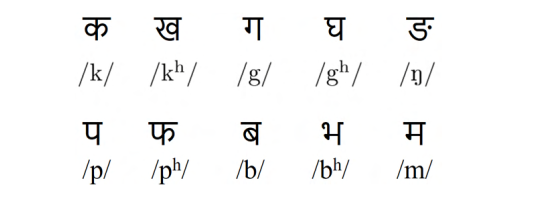
\includegraphics[width=0.6\textwidth]{Figs/Q36.png}
\caption{}
\label{fig:3.4}
\end{figure}
\begin{enumerate} \begin{multicols}{2}
\item Voicing
\item Manner of articulation
\item Place of articulation
\item Aspiration
\end{multicols} \end{enumerate}
\hfill\brak{GATE \ XH \ 2023}
%Q.37
\item Which option is related to Neo-Whorfism?
\begin{enumerate} 
\item Language, thought, worldview
\item Innateness, deep-structure, surface-structure
\item Language, methods, analysis
\item Signifier, signified, sign
\end{enumerate}
\hfill\brak{GATE \ XH \ 2023}
%Q.38
\item Which of the following is/are involved in the comparative method for establishing language families and genetic relationship among languages?
\begin{enumerate} 
\item Reconstruction of the proto language
\item Assembling a list of cognates
\item Strictly using basic vocabulary lists
\item Setting up sound correspondences
\end{enumerate}
\hfill\brak{GATE \ XH \ 2023}
%Q.39
\item Aphasia can be caused by
\begin{enumerate} 
\item Open or closed head trauma
\item Attention deficit
\item Neurodegeneration in advanced age
\item Lack of motivation
\end{enumerate}
\hfill\brak{GATE \ XH \ 2023}
%Q.40
\item In sociolinguistics, the term ‘anti-language’ refers to the language used for
\begin{enumerate} 
\item Academic purposes by professional criminologists
\item Legal proceedings in the court of law
\item Communication by small non-mainstream groups
\item Communication between caregivers and infants
\end{enumerate}
\hfill\brak{GATE \ XH \ 2023}
%Q.41
\item In language policy making, which of the following steps is/are necessary for an erstwhile minority language, spoken by a sizeable population, to be introduced as a medium of instruction in schools?
\begin{enumerate} 
\item Language revival
\item Corpus planning
\item Status planning
\item Language preservation
\end{enumerate}
\hfill\brak{GATE \ XH \ 2023}
%Q.42
\item Which of the following research methods involve Reaction Time?
\begin{enumerate} 
\item Behavioral methods
\item Experimental methods
\item Non-behavioral methods
\item Qualitative methods
\end{enumerate}
\hfill\brak{GATE \ XH \ 2023}
%Q.43
\item If \sbrak{p} and $\sbrak{p^h} $ are allophones of the same phoneme /p/, which of the following statements is/are true?
\begin{enumerate} 
	\item \sbrak{p} and $\sbrak{p^h} $ are in contrastive distribution
	\item \sbrak{p} and $\sbrak{p^h} $ are in complementary distribution
	\item $\sbrak{p^h} $ has more restrictive occurrence than \sbrak{p}
	\item \sbrak{p} and $\sbrak{p^h} $ can be used interchangeably
\end{enumerate}
\hfill\brak{GATE \ XH \ 2023}
%Q.44
\item Which of the following show(s) dissociation between cognitive disorder and language abilities?
\begin{enumerate} 
\item Autism spectrum disorder
\item Williams syndrome
\item Dyslexia
\item Specific Language Impairment (SLI)
\end{enumerate}
\hfill\brak{GATE \ XH \ 2023}
\newpage
\textbf{XH-C3: Q.45 – Q.65 Carry TWO marks Each}
%Q.45
\item Which of the following sound pairs differ from each other in exactly two articulatory parameters?
\begin{enumerate} \begin{multicols}{2}
	\item \sbrak{p} vs. \sbrak{b}
	\item \sbrak{t} vs. \sbrak{s}
	\item \sbrak{v} vs. $\sbrak{\theta} $
	\item \sbrak{n} vs. \sbrak{d}
\end{multicols} \end{enumerate}
\hfill\brak{GATE \ XH \ 2023}
%Q.46
\item The cover term determiner refers to:
\begin{enumerate} 
\item Articles, demonstratives, and possessors
\item Possessors, prepositions, and demonstratives
\item Postpositions, articles, and prepositions
\item Articles, prepositions, and possessors
\end{enumerate}
\hfill\brak{GATE \ XH \ 2023}
%Q.47
\item In ‘John seems to have left’, the subject John has undergone:
\begin{enumerate} 
\item Subject-to-Subject lowering
\item Object-to-Subject raising
\item Subject-to-Subject raising
\item Object-to-Object lowering
\end{enumerate}
\hfill\brak{GATE \ XH \ 2023}
%Q.48
\item The comparative and superlative forms of the adjective ‘good’ are examples of:
\begin{enumerate} \begin{multicols}{2}
\item Alternation
\item Syncope
\item Ablaut
\item Suppletion
\end{multicols} \end{enumerate}
\hfill\brak{GATE \ XH \ 2023}
%Q.49
\item Consider the following question and determine where was is moved finally, in accordance with the minimalist assumptions: Was John, who wrote the book, angry?
\begin{enumerate} \begin{multicols}{2}
\item T to C
\item C to T
\item V to T
\item T to V
\end{multicols} \end{enumerate}
\hfill\brak{GATE \ XH \ 2023}
%Q.50
\item Match the following historical sound changes in Column X with the processes in Column Y
\begin{table}[H]
    \centering
\begin{tabular}{|l|l|}
        \hline
        Column X & Column Y \\
        \hline
        P. r\={u}pa $\rightarrow$ r\={u}p & 1. Grassmann's law \\
        Q. sapta $\rightarrow$ satta & 2. Apocope \\
        R. b$^h$od$^h$a $\rightarrow$ bod$^h$a & 3. Assimilation \\
        S. sa\d{m}kalana $\rightarrow$ sa\.{n}kalana & 4. Compensatory lengthening \\
        \hline
    \end{tabular}

    \caption{}
    \label{tab:ling_q50}
\end{table}
\begin{enumerate} 
\item P-2, Q-4, R-1, S-3
\item P-4, Q-2, R-1, S-3
\item P-2, Q-1, R-4, S-3
\item P-2, Q-4, R-3, S-1
\end{enumerate}
\hfill\brak{GATE \ XH \ 2023}
%Q.51
\item Consider the following morphological break-up of pfeifing produced by a simultaneous bilingual child. What phenomenon does this example indicate?
\begin{center}
pfeife + ing $\rightarrow$ pfeifing \\
whistle (German) + progressive (English) $\rightarrow$ ‘whistling’
\end{center}
\begin{enumerate} 
\item Code-mixing arising out of social bilingualism
\item Code-switching based on context of the conversation
\item Understanding both languages as part of a single ‘system’
\item Mixed language arising out of pedagogical preferences
\end{enumerate}
\hfill\brak{GATE \ XH \ 2023}
%Q.52
\item Which one of the following is compounding of compounded words?
\begin{enumerate} \begin{multicols}{2}
\item Lighthouse tower
\item Skating board
\item Boyfriend
\item Walkman
\end{multicols} \end{enumerate}
\hfill\brak{GATE \ XH \ 2023}
%Q.53
\item What sociolinguistic phenomenon does the following sentence exemplify?

\begin{center}
\begin{tabular}{lllll}
    la & fam & \textbf{micimine:w} & li & pci \\
    the\brak{fem.} & woman & \textbf{she-is-holding-it} & the \brak{masc.} & little-one \\
    French & French & \textbf{Cree} & French & French \\[2ex]
    \multicolumn{5}{c}{“The woman is holding the child”} \\
\end{tabular}
\end{center}

\begin{enumerate}
    \begin{multicols}{2}
        \item Code switching
        \item Bilingualism
        \item Pidgin
        \item Mixed language
    \end{multicols}
\end{enumerate}
\hfill\brak{GATE \ XH \ 2023}
%Q.54
\item Identify the labels for X and Y in the following tree.
\begin{figure}[H]
\centering
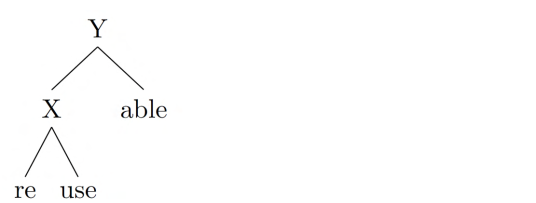
\includegraphics[width=0.2\textwidth]{Figs/Q54.png}
\caption{}
\label{fig:3.5}
\end{figure}
\begin{enumerate} 
\item X: Verb, Y: Adjectivei
\item X: Adjective, Y: Adjective
\item X: Adjective, Y: Verb
\item X: Verb, Y: Verb
\end{enumerate}
\hfill\brak{GATE \ XH \ 2023}
%Q.55
\item From the following, which is the correct order of animacy hierarchy?
\begin{enumerate} 
\item 1st/2nd Person $>$ 3rd Person $>$ Proper Name $>$ Human Noun
\item 3rd Person $>$ 1st/2nd Person $>$ Proper Name $>$ Human Noun
\item 3rd Person $>$ 1st/2nd Person $>$ Human Noun $>$ Proper Name
\item 1st/2nd Person $>$ 3rd Person $>$ Human Noun $>$ Proper Name
\end{enumerate}
\hfill\brak{GATE \ XH \ 2023}
%Q.56
\item Look at the adjectives in Column X and match with the types of adjectives in Column Y. Choose the correct option.
\begin{table}[H]
    \centering 
\begin{tabular}{|l|l|}
        \hline
	Column X & Column Y \\
        \hline
        P. Blue shirt & 1. Subsective \\
        Q. Fake Picasso & 2. Intersective \\
        R. Big elephant & 3. Anti-intersective \\
        \hline
    \end{tabular}

    \caption{}
    \label{tab:ling_q56}
\end{table}
\begin{enumerate} 
\item P-2, Q-3, R-1
\item P-2, Q-1, R-3
\item P-1, Q-2, R-3
\item P-1, Q-3, R-2
\end{enumerate}
\hfill\brak{GATE \ XH \ 2023}
%Q.57
\item In a given constraint ranking of \textbf{COMPLEX, DEP-IO $>>$ MAX-IO} for the input /spun/, which of the following candidates is/are optimal?
\begin{enumerate} \begin{multicols}{2}
\item \sbrak{su.pun}
\item \sbrak{pun}
\item \sbrak{sun}
\item \sbark{is.pun}
\end{multicols} \end{enumerate}
\hfill\brak{GATE \ XH \ 2023}
%Q.58
\item Consider the pattern of stress assignment shown below. Which of the given statements is/are true?
	\newline
    \vspace{0.5em}
    \hspace*{1.5em} * \\[0.2ex]
    \hspace*{1.5em} * \hspace{3.5em} * \\[0.2ex]
    \hspace*{1.5em} * \hspace{3.5em} * \\[1ex]
	\brak{ma . pi} \hspace{1em} \brak{le . se} \hspace{1em} $<gu>$
    \vspace{0.5em}
\begin{enumerate} 
\item Stress assignment is from left to right
\item There are/is extrametrical syllable(s)
\item Feet are binary
\item Stress system is iambic
\end{enumerate}
\hfill\brak{GATE \ XH \ 2023}
%Q.59
\item In word processing studies, visual word recognition is affected by:
\begin{enumerate} 
\item Proficiency, word length, neighborhood effect
\item Frequency, age of acquisition \brak{AoA}, familiarity
\item McGurk effect, place and manner of articulation \brak{PoA and MoA}
\item Language family, areal features, phoneme inventory size
\end{enumerate}
\hfill\brak{GATE \ XH \ 2023}
%Q.60
\item Identify the language(s) that belong(s) to the Balkan Sprachbund.
\begin{enumerate} \begin{multicols}{4}
\item Romanian
\item Bulgarian
\item Norwegian
\item Swedish
\end{multicols} \end{enumerate}
\hfill\brak{GATE \ XH \ 2023}
%Q.61
\item Consider the following tree structure, where A and C are co-referential. Similarly, E and H are co-referential. Identify the incorrect statement(s).
\begin{figure}[H]
\centering
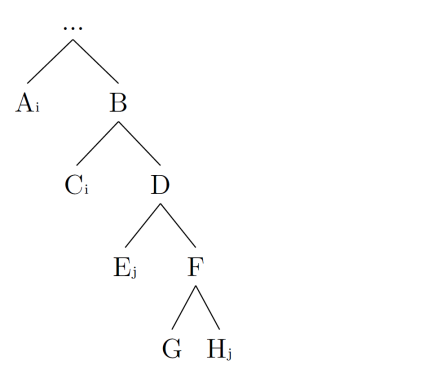
\includegraphics[width=0.25\textwidth]{Figs/Q61.png}
\caption{}
\label{fig:3.6}
\end{figure}
\begin{enumerate} \begin{multicols}{4}
\item A binds C
\item C binds E
\item E binds D
\item A binds H
\end{multicols} \end{enumerate}
\hfill\brak{GATE \ XH \ 2023}
%Q.62
\item Which of the following statements is/are true for the pair - bird : cuckoo
\begin{enumerate} 
\item Cuckoo is the hyponym of bird
\item Bird is the hypernym of cuckoo
\item Cuckoo is the hypernym of bird
\item Bird is the hyponym of cuckoo
\end{enumerate}
\hfill\brak{GATE \ XH \ 2023}
%Q.63
\item In the sentences 1 through 4, in which one(s) a) entails b)?
\begin{multicols}{2}
    \begin{enumerate}
        \item 
        \begin{enumerate}[topsep=0pt, itemsep=0pt, parsep=0pt]
            \item Rama plays a string instrument.
            \item Rama is a violinist.
        \end{enumerate}

        \item 
        \begin{enumerate}[topsep=0pt, itemsep=0pt, parsep=0pt]
            \item Hutolu sings.
            \item Hutolu is melodious.
        \end{enumerate}
        
        \columnbreak

        \item 
        \begin{enumerate}[topsep=0pt, itemsep=0pt, parsep=0pt]
            \item Fido is a Dalmatian.
            \item Fido is a dog.
        \end{enumerate}

        \item 
        \begin{enumerate}[topsep=0pt, itemsep=0pt, parsep=0pt]
            \item Students don't study.
            \item Linguistics students do not study.
        \end{enumerate}
    \end{enumerate}
\end{multicols}
\begin{enumerate}
    \begin{multicols}{2}
        \item 1 a) entails 1 b)
        \item 2 a) entails 2 b)
        \item 3 a) entails 3 b)
        \item 4 a) entails 4 b)
    \end{multicols}
\end{enumerate}
\hfill\brak{GATE \ XH \ 2023}
%Q.64
\item The following figure depicts a spectrum of a vowel (dashed line), where F0 = 150 Hz and F0 = H1. The harmonics are indicated from H1 to H11. From the figure, the frequency (in Hz) of the second formant (F2) of this vowel is\_\_\_\_\_\_.
\begin{figure}[H]
\centering
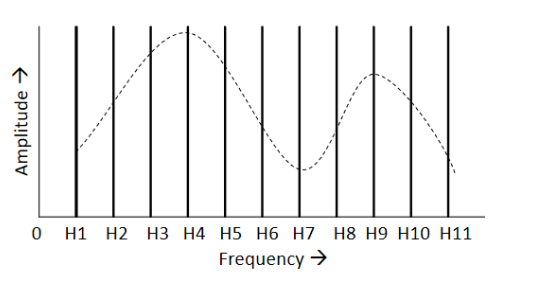
\includegraphics[width=0.6\textwidth]{Figs/Q64.png}
\caption{}
\label{fig:3.7}
\end{figure}
\hfill\brak{GATE \ XH \ 2023}
%Q.65
\item The number of core arguments associated with the ditransitive verb ‘give’ is \_\_\_\_\_\_\_.
\hfill\brak{GATE \ XH \ 2023}
\end{enumerate}
\end{document}
